% ****** Start of file dressed_quantum_hall.tex ****** %

\documentclass[
 reprint,
 amsmath,amssymb,
 aps,
 prb,
]{revtex4-2}

%===============================================================================
% Import packages
%===============================================================================
% Bold math
\usepackage{bm}
% AMS packages
\usepackage{amsfonts}
\usepackage{amsmath}
\usepackage{amssymb}
\usepackage{mathtools}
% Physics package
\usepackage{physics}
% SI units package
\usepackage{siunitx}
% Hypertext package
\usepackage[breaklinks=true,colorlinks=true,linkcolor=blue,urlcolor=blue,citecolor=blue]{hyperref}
% Language and font encodings
\usepackage[english]{babel}
\usepackage[utf8x]{inputenc}
\usepackage[T1]{fontenc}
%===============================================================================
% Bibliography style
\bibliographystyle{apsrev4-2}

\begin{document}

\preprint{APS/123-QED}

% Title of the manuscript
\title{A generalized model for the charge transport properties of
\\dressed quantum Hall systems}

% Authors of the manuscript
\author{Kosala Herath,}
\email[]{kosala.herath@monash.edu}
\author{Malin Premaratne}
\email[]{malin.premaratne@monash.edu}
\affiliation{Advanced Computing and Simulation Laboratory (A$\chi$L), Department of Electrical and Computer Systems Engineering, Monash University, Clayton, Victoria 3800, Australia.}

% Add date
\date{\today}

% Abstract
\begin{abstract}
A generalized mathematical model for the transport properties of systems exposed to a stationary magnetic and a strong electromagnetic field is presented. The new formulation, which applies to the two-dimensional dressed quantum Hall systems, is based on Landau quantization theory and Floquet-Drude conductivity method. We model our system as a two-dimensional electron gas (2DEG) that interacts with two external fields. To incorporate the strong light coupling with the 2DEG, we utilize the Floquet theory to analyze the effect non perturbatively. Moreover, the Floquet Fermi "golden rule" is adopted to explore the scattering effects for Floquet states in disordered quantum Hall systems. Based on our fully analytical expression and particular graphical representations, we demonstrate
that the characteristics of conductivities in two-dimensional quantum Hall systems can manipulate using a dressed field. The outcomes align with theoretical descriptions which are already well-suited with experimental results at the same time our theory provides a more generalized analysis on the properties of conductivity in quantum Hall systems. Thus, this model more realistically describes that how to use external strong radiation as a tool to utilize transport properties in various 2D nanostructures which serve as a basis for nano-optoelectronic devices.

\end{abstract}

% Make title of the manuscript
\maketitle

% Section 01 : Introduction
\section{\label{sec_introduction} Introduction}
% Section 01 - Introduction

Manipulating light-matter interactions in the quantum regime paved the path for an astonishing number of useful technologies in the last century. Quantum optics, which study these interactions, have drawn research attention to the disciplines of optoelectronics \cite{liu16,wijesekara20,tao21,wijesekara21}, sensing \cite{rodrigo2015,pirandola18,hapuarachchi2018}, energy harvesting \cite{yuan16,sun18},
quantum computing \cite{huh15,slussarenko19,andersen21}, bio-information \cite{marais18,bian20}, and many other specialities of recent technologies \cite{rivera20}.
The studies on quantum optics of nanostructures were generally centered on metamaterials \cite{shalaev07,si14}, quantum plasmonic effects \cite{hapuarachchi19,perera20}, lasers and amplifiers \cite{zhang05,chow13}, and quantum cavity physics \cite{tsang10,devi20}.
However, in recent years, one of the foremost aim of examining nanostructures under external radiation was understanding their electron transport characteristics \cite{kitagawa11,zhou11,kibis14,pervishko15,morina15,dehghani15,dini16,wackerl20}.

Better understanding the fundamental mechanisms of charge transport can allow us to invent novel nanoelectronic devices and optimize their performance \cite{premaratne21}.
Most recent studies on the subject have considered the driving field as a perturbation field \cite{pervishko15,morina15}. However, this assumption breaks down for systems under high-intensity illuminations \cite{grifoni98,wackerl20}.
Modeling an electromagnetic field under a perturbative formalism involves expanding the interaction terms in powers of the field intensity. At high intensities, the higher-order terms influence the physics more strongly and the basis of the perturbative treatment begins to break down.
In these instances, a more accurate treatment needs to be adopted. Thus, we treat the interacting fermion system and the radiation as one combined quantum system, namely dressed system \cite{morina15,cohen98,scully01}. Here the applied high-intensity  electromagnetic field identify as the dressing field.

Theoretical analyses on the transport properties of dressed fermion systems were recently reported in Refs. \cite{kibis14,morina15,wackerl20}.
Furthermore, in Ref. \cite{wackerl20} a general expression for conductivity in a dressed system has been derived in a fully closed analytical form. In their study, a novel type of Green’s functions, namely four-times Green’s functions were used to derive the Floquet-Drude conductivity formula. This opened the path to exploring and exploiting nanostructures' charge transport attributes under an intense dressing field.

Quantum Hall effect \cite{girvin90} observed in two-dimensional (2D) fermion systems at low temperatures under strong stationary magnetic fields manifest remarkable magneto-transport behaviors. Transport properties of these systems have recently attracted both theoretical \cite{ando72,ando74_1,ando74_2,ando74_3,ando74_4,ando82,endo09} and experimental \cite{allerman95,tieke97,pan05} interest.
Endo \textit{et al.} \cite{endo09} presented the calculations of longitudinal and transverse conductivity tensor components and their relationship in a quantum Hall system. These theoretical calculations  align better with experimental observations compared to previous studies.

In contrast, more exciting phenomena can be observed by simultaneously applying a dressing field to a quantum Hall system already under a non-oscillating magnetic field.
Whilst there exist several leading theories for calculating conductivity tensor elements in quantum Hall systems \cite{ando74_1,ando82,endo09}, they have not been utilized to describe the optical manipulation of charge transport.
Recently, Dini \textit{et al.} \cite{dini16} have investigated the one-directional conductivity behavior of dressed quantum Hall systems. However, they have not adopted the state-of-the-art model to describe the conductivity in a quantum Hall system. In their study, they used the conductivity models from Refs. \cite{ando74_1,ando82}, and as mentioned in Endo \textit{et al.} \cite{endo09}, those models predict a semi-elliptical broadening against Fermi level for each Landau level and provide less agreement with the empirical results.

In the present analysis, we present a robust mathematical model for a dressed two-dimensional electron gas (2DEG) subject to another nonoscillating magnetic field.
A stationary magnetic field is applied perpendicularly across the surface of the 2DEG system. This causes the orbital motion of the electrons to be quantized, and a discrete energy spectrum with Landau splitting is observed \cite{landau30}.
In this study, we explicitly calculate the longitudinal components ($\sigma^{xx},\sigma^{yy}$) of the conductivity tensor in a periodically driven quantum Hall system by developing a generalized analytical description using the Floquet-Drude conductivity \cite{wackerl20}.
Finally, we demonstrate that our generalized model reproduces the results of the state-of-the-art conductivity model in Ref. \cite{endo09}, which was developed for the more specific case of quantum Hall systems without the external dressing field.
Moreover, we find that the optical field can be used as a mechanism to regulate transport behavior in numerous 2D nanostructures which can serve as a basis for many useful nanoelectronic devices. We believe that our theoretical analysis and visual depictions of numerical results will lead to a better understanding of manipulating charge transport. Moreover, this will inspire advanced  developments in nanoscale quantum devices.

The paper is organized as follows. Sec.  \ref{sec_schrodinger_problem} introduces our dressed quantum Hall system and the exact wave function solutions for the given configuration. Sec. \ref{sec_floquet_theory} provides the Floquet theory interpretation of these wave functions.
We introduce Floquet-Fermi golden rule for a quantum Hall system in Sec. \ref{sec_inverse_scattering_time}, and use it in Sec. \ref{sec_floquet_drude_conductivity} to derive analytical expressions for longitudinal components of conductivity.
The derived theoretical model is further analyzed numerically using empirical system parameters and compared with previous studies in Sec. \ref{sec_manipulate_conductivity}.
In Sec. \ref{sec_conclusions}, we summarize our analysis and present our conclusions.


% Section 02 : Schrodinger problem for a dressed quantum Hall system
\section{\label{sec_schrodinger_problem} Schrodinger problem for a dressed quantum Hall system}
% Section 02 - Schrodinger problem for dressed quantum Hall system

Our system consist of a two-dimentional free electron gas (2DEG) confined in the $(x,y)$ plane of the three-dimentional coordinate space. In our analysis, the 2DEG is subjected to a stationary magnetic field $\vb{B} = (0,0,B)^{\text{T}}$ which is pointed towards the $z$ axis. In addition, a linearly polarized strong light is applied perpendicular to the 2DEG plane, and we specially tune the frequency of the field $\omega$ such that the optical field behaves as a purely dressing field (unabsorbable). Without limiting the generality we can choose $y$-polorized electric field $\vb{E} = (0,E\sin(\omega t),0)^{\text{T}}$ for the dressing field configuration (Fig.~\ref{fig_1}).
\begin{figure}[b]
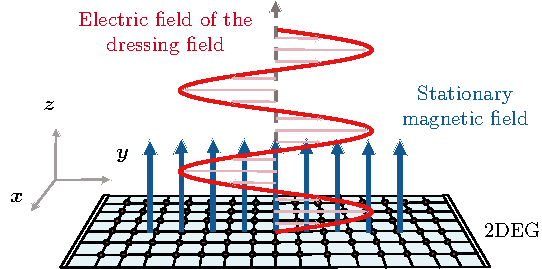
\includegraphics[scale=0.9]{figures/fig_1}
\caption{\label{fig_1} Two-dimensional electron gas (2DEG) confined in the $(x,y)$ plane while both stationary magnetic field $\vb{B}$ and strong dressing field with y-polarized electric field $\vb{E}$ are being applied perpendicular to the surface of 2DEG.}
\end{figure}
Here $B$ and $E$ represent the amplitude of the stationary magnetic field and oscillating electric field respectively.

Using Landau gauge for the stationary magnetic field, we can represent it using vector potential as $\vb{A}_{s} = (-By,0,0)^{\text{T}}$ and choosing Coulomb gauge, the vector potential of the dynamic dressing radiation can be presented as $\vb{A}_{d}(t) = (0,[E/\omega ]\cos(\omega t),0)^{\text{T}}$. These vector potentials are coupled to the momentum of 2DEG as kinetic momentum \cite{mahan00,bruus04} and this leads to the time-dependent Hamiltonian
\begin{equation} \label{eq_1}
  \hat{H}_e(t) = \frac{1}{2m_e}\Big[\hat{\vb{p}} - e\big(\vb{A}_{s}+\vb{A}_{d}(t)\big)\Big]^2,
\end{equation}
where $m_e$ is the effective electron mass and $e$ is the magnitude of the electron charge. $\hat{\vb{p}} = (\hat{p}_x,\hat{p}_y,0)^{\text{T}}$ represents the canonical momentum operator for 2DEG with electron momentum $p_{x,y}$.
The exact solutions for the time-dependent Schrödinger equation $i\hbar \dv{t}\psi = \hat{H}_e(t) \psi$ was already given by Refs. \cite{husmi53,ditt98,dini16} and we can present them as a set of wave functions defined by two quantum numbers $(n,m)$
\begin{equation} \label{eq_2}
  \begin{aligned}
    \psi_{n,m}&(x,y,t)  \\
    & = \frac{1}{\sqrt{L_x}}
    \chi_n\left[y - y_0 - \zeta(t)\right]\\
    & \times
    \text{exp}\bigg(
    \frac{i}{\hbar}\bigg[- \varepsilon_nt
    + p_x x + \frac{eE(y - y_0)}{\omega}\cos(\omega t)\\
    &+
    m_e\dot{\zeta}(t)\big[y - y_0 -\zeta(t)\big] +
    \int_0^{t}dt'L(\zeta,\dot{\zeta},t')\bigg]\bigg),
  \end{aligned}
\end{equation}
where $n \in \mathbb{Z}^{+}_0$ and $m \in \mathbb{Z}$ ; see Appendix A. Here $L_{x,y}$ are dimension of the 2DEG surface, $\hbar$ is the reduced Planck constant, and $y_0 = -p_x/eB$ is the center of the cyclotron orbit along $y$ axis. $\chi_n$ are well known solutions for Schrödinger equation of a stationary quantum harmonic oscillator
\begin{equation} \label{eq_3}
  \chi_n(x) \equiv
   \frac{\sqrt{\kappa}}{\sqrt{2^{n}n!}}
  e^{-\kappa^2 x^2/2}
  \mathcal{H}_n \qty(\kappa x) \quad \text{with}
  \quad
  \kappa = \sqrt{\frac{m_e \omega_0}{\hbar}},
\end{equation}
with eigenvalues given by $\varepsilon_n = \hbar \omega_0 (n + 1/2)$ and $\omega_0 = eB/m_e$ is the cyclotron frequency. Each $n$ value defines the  energy($\varepsilon_n$) of the respective Landau level. The path shift of the driven classical oscillator $\zeta(t)$ is given by
\begin{equation} \label{eq_4}
  \zeta(t) = \frac{eE}{m_e(\omega_0^2 - \omega^2)}\sin(\omega t),
\end{equation}
while the Lagrangian of the classical oscillator $L(\zeta,\dot{\zeta},t)$ can be identified as
\begin{equation} \label{eq_5}
  L(\zeta,\dot{\zeta},t) = \frac{1}{2} m_e\dot{\zeta}^2(t) - \frac{1}{2}m_e\omega_0^2 \zeta^2(t) + eE\zeta(t) \sin(\omega t).
\end{equation}
The exponential phase shifts in Eq.~(\ref{eq_2}) represent the influence done by the stationary magnetic field and strong dressing field. Therefore, we can accept that magneto-transport properties of 2DEG will be renormalized by the magnetic field as well as the dressing field.


% Section 03 : Floquet theory perspectiv
\section{\label{sec_floquet_theory} Floquet theory perspective}
Considerable research effort in recent years has been de- voted to synthesizing materials whose thermal conductivity.


% Section 04 :
\section{\label{sec_inverse_scattering_time}  Inverse Scattering Time Analysis}
% Section 04 - Inverse Scattering Time Analysis

The Floquet-Fermi golden rule was proposed in Ref. \cite{wackerl20} as an approach to analyze the transport properties of dressed quantum systems with impurities.
However, this theory has not been applied for a dressed quantum Hall system in the previous studies. In this analysis, we use Floquet-Fermi golden rule to identify the effects induced by impurities on the magneto-transport properties.
With the help of $t-t'$ formalism \cite{wackerl20,grifoni98,sambe75,peskin93,althorpe97} and applying Floquet states derived in Eq.~(\ref{eq_12}), we can derive an  expression for $(l,l')$-th element of the inverse scattering time matrix for the $N$-th Landau level as
\begin{equation} \label{eq_13}
  \begin{aligned}
    \bigg(&\frac{1}{\tau(\varepsilon,k_x)}\bigg)^{ll'}_{N} \\
    & =
    \frac { \varrho^2}{eB}
    \delta(\varepsilon - \varepsilon_{N}) \\
    & \quad\times
    \int_{-\infty}^{\infty} d k_1 \Bigg[
    J_l\qty(\frac{b\hbar}{eB}[{k}_x - k_1])
    J_{l'}\qty(\frac{b\hbar}{eB}[{k}_x - k_1]) \\
    & \quad\times
    \qty|
    \int_{-\infty}^{\infty} dk_2 \;
    {\chi}_{N}\qty(\frac{\hbar}{eB}k_2)
    {\chi}_{N}\qty(\frac{\hbar}{eB} \qty[k_1 - {k}_x - k_2])|^2\Bigg],
  \end{aligned}
\end{equation}
where $\varrho = \eta_{imp} L_x [ { V_{imp}}/{eB}]^{1/2}$, $\varepsilon$ is a given energy value, $J_l(\cdot)$ are Bessel functions of the first kind with $l$-th integer order, and $\varepsilon_N$ is the energy of the $N$-th Landau level.
A more detailed derivation is given in Appendix \ref{appendix_c}.
We modeled the effect caused by impurities in the considered system as a single perturbation potential.
Since random impurities in a disordered metal offers a better approximation for experimental conditions, we assumed that our perturbation potential is formed by a group of randomly distributed impurities.
Thus, the total scattering potential in the 2DEG has been represented as a sum of uncorrelated single impurity potentials $\upsilon(\vb{r})$. Here $\eta_{imp}$ is the number of impurities in a unit area, $V_{imp} = \expval{|V_{{k'}_x,k_x}|^2}_{imp}$ with $V_{{k'}_x,k_x} = \mel**{k'_x}{\upsilon(x) }{k_x}$, and $\braket{x}{k_x} = e^{-ik_x x}$.
Moreover in this analysis, $\expval{\cdot}_{imp}$ represents the average over the impurity disorder.

Next, we analyze the contribution of the inverse scattering time matrix elements on the transport properties of our system.
Since the disorder in the system can not singificantly alter the eigenenergy values of the undressed system \cite{wackerl20}, we can neglect the contribution of all off-diagonal elements in the inverse scattering time matrix. Subsequenty we consider only the central (${l=l'=0}$) diagonal element of the inverse scattering time matrix which has the largest contribution to the transport characteristics. Along with this assumption, we introduce a new parameter as the scattering-induced broadening of the $N$-th Landau level \cite{dini16,endo09}
\begin{equation} \label{eq_14}
 \Gamma^{00}_{N}(\varepsilon,k_x) = \hbar \qty(\frac{1}{\tau(\varepsilon,k_x)})^{00}_{N},
\end{equation}
which simplifies to
\begin{equation} \label{eq_15}
 \begin{aligned}
   &\Gamma^{00}_{N} (\varepsilon,k_x) \\
   & =
   \frac { \varrho^2}{eB}
   \delta(\varepsilon - \varepsilon_{N}) \\
   & \quad\times
   \int_{-\infty}^{\infty} d k_1 \Bigg[
   J_0^2\qty(\frac{b\hbar}{eB}[{k}_x - k_1])
   \\
   & \quad\times
   \qty|
   \int_{-\infty}^{\infty} dk_2 \;
   {\chi}_{N}\qty(\frac{\hbar}{eB}k_2)
   {\chi}_{N}\qty(\frac{\hbar}{eB} \qty[k_1 - {k}_x - k_2])|^2\Bigg].
 \end{aligned}
\end{equation}

\begin{figure}[t]
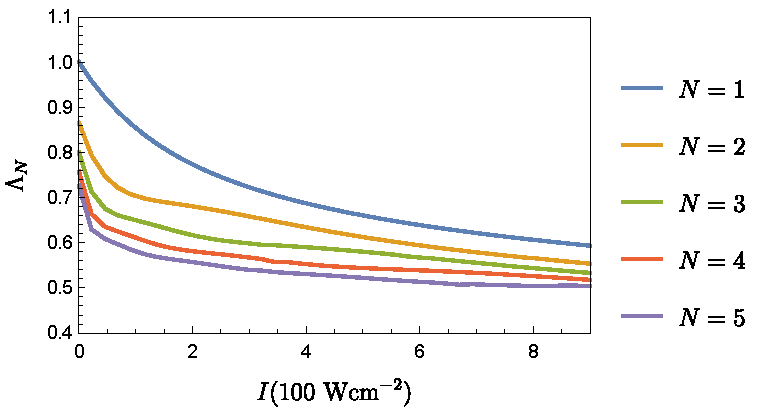
\includegraphics[scale=0.68]{figures/fig_3}
\caption{\label{fig_3} The dependence of normalized scattering-induced broadening $\Lambda_N$ for each Landau level ($N =0,1,2,3,4$) against $x$-directional momentum value $k_x$ in a GaAs-based quantum well under a nonoscillating magnetic field with $B = 1.2~\text{T}$, dressing field with frequency of $\omega =2\times10^{12}~\text{rad}\text{s}^{-1}$ and intensity $I =100~\text{W}/\text{cm}^{2}$.
In this calculation we have assumed that the natural  broadening of $0$-th Landau level $\Gamma_0$ is $0.24\;\text{me}V$.}
\end{figure}

\begin{figure}[b]
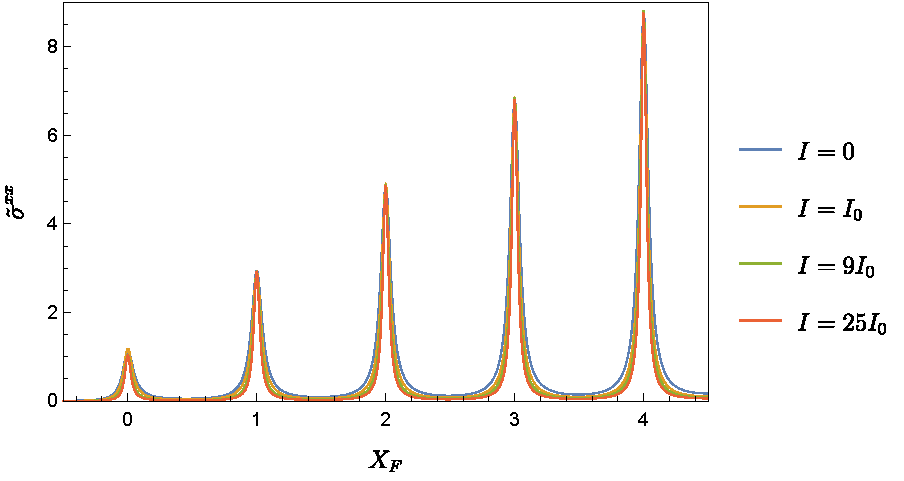
\includegraphics[scale=0.68]{figures/fig_4}
\caption{\label{fig_4} The dependence of normalized scattering-induced broadening $\Lambda_N$ for each Landau level ($N =0,1,2,3,4$) against dressing field intensity $I$, in a GaAs-based quantum well under a nonoscillating magnetic field with $B = 1.2~\text{T}$, dressing field with frequency of $\omega =2\times10^{12}~\text{rad}\text{s}^{-1}$. In this calculation we have assumed that the natural broadening of $0$-th Landau level $\Gamma_0$ is $0.24\;\text{me}V$.}
\end{figure}

In addition, for a scattering scenario taking place wihtin the same Landau level, we are able to present the delta distribution of the energy by the  interpretation \cite{dini16}
\begin{equation} \label{eq_16}
 \delta(\varepsilon - \varepsilon_{N}) \approx
 \frac{1}{\pi \Gamma^{00}_{N}(\varepsilon,k_x)}.
\end{equation}
Then we write the central element of inverse scattering time matrix in the more compact form
\begin{equation} \label{eq_17}
  \begin{aligned}
    \Gamma^{00}_{N}(\varepsilon,& k_x) =
    \varrho
    \bigg[
    \int_{-\infty}^{\infty} d {k}_1 \;
    J_0^2\qty(\lambda_1[{k}_x - {k}_1]) \\
    & \times
    \qty|
    \int_{-\infty}^{\infty} d{k}_2 \;
    \tilde{\chi}_{N}\qty(\lambda_2 k_2)
    \tilde{\chi}_{N}\qty(\lambda_2 \qty[{k}_1 - {k}_2 - {k}_x])|^2
    \bigg]^{-\frac{1}{2}},
  \end{aligned}
\end{equation}
where $ \lambda_1 \equiv \hbar b/eB$ and  $\lambda_2 \equiv \hbar \kappa/eB$.
To analyze the effects of the dressing field on the scattering-induced broadening, we introduce the normalized $N$-th Landau level scattering-induced broadening as
\begin{equation} \label{eq_18}
    \Lambda_N(k_x) =
    \frac{\Gamma^{00}_{N}(\varepsilon,k_x)}{\Gamma^{00}_{N=0}(\varepsilon,k_x)\big|_{E=0}},
\end{equation}
which can be evaluated with
\begin{widetext}
\begin{equation} \label{eq_19}
    \Lambda_N (k_x) =
    \qty[
    \frac
    {\int_{-\infty}^{\infty} d {k}_1 \;
    J_0^2\qty(\lambda_1[{k}_x - {k}_1])
    \qty|
    \int_{-\infty}^{\infty} d{k}_2 \;
    \tilde{\chi}_{N}\qty(\lambda_2 k_2)
    \tilde{\chi}_{N}\qty(\lambda_2 \qty[{k}_1 - {k}_2 - {k}_x])|^2}
    {\int_{-\infty}^{\infty} d {k}_1 \;
    \qty|
    \int_{-\infty}^{\infty} d{k}_2 \;
    \tilde{\chi}_{0}\qty(\lambda_2 k_2)
    \tilde{\chi}_{0}\qty(\lambda_2 \qty[{k}_1 - {k}_2 - {k}_x])|^2}
    ]^{1/2}.
\end{equation}
\end{widetext}

Normalized energy band broadening against x-directional momentum component ${k_x}$ for different Landau levels ($N = 0,1,2,3,4$) has been calculated for GaAs-based quantum well and the results are depicted in Fig.~(\ref{fig_3}) and Fig.~(\ref{fig_4}). To make a comparison, we have selected the experiment parameters to match with analysis in Ref.~\cite{endo09}.
In that study, the authors have assumed that effective mass of the electron in GaAs-based quantum well system is $m_e \approx 0.07\tilde{m}_e$ where $\tilde{m}_e$ is mass of the electron \cite{endo09,winkler03,wackerl20}. In addition, they used the broadening of the undressed $0$-th Landau level $\Gamma_0$ as $0.24\;\text{me}V$. Therefore, in our calculations, we assumed that the natural least Landau level broadening also has this value: $\Gamma^{00}_{N=0}|_{E=0} = 0.24 \;\text{meV}$.
Here, we observe that the normalized energy broadening value for each Landau level is independent of the x-directional momentum $k_x$ value and we are able to manipulate it by the dressing field. When the dressing field's intensity increases, the energy broadening is reduced, which leads to changes in the transport properties of the dressed quantum Hall system.
To analyze these adjustments in detail, we derive a analytical expression for the conductivity of a dressed quantum Hall system in the next section.


% Section 05 :
\section{\label{sec_floquet_drude_conductivity} Floquet-Drude Conductivity in a Dressed Quantum Hall System}
% Section 05 - Floquet-Drude Conductivity in Quantum Hall Systems

A general theory for the conductivity of a dressed system with the disorder was reported by Wackerl \textit{et al.} \cite{wackerl20,wackerlthesis20}. This theory, the general $x$-directional longitudinal DC-limit conductivity has been characterized as
\begin{equation} \label{eq:22}
  \begin{aligned}
    \sigma^{xx} = &
    \frac{-1}{4\pi\hbar A}
    \int_{\Pi-\hbar\omega/2}^{\Pi+ \hbar\omega/2}
    \left(
    -\pdv*{f}{\varepsilon }\right) \\
    &  \quad\times
    \tr
    \left\{
    {j}^x_0
    \left[
    \vb{G}^{r} (\varepsilon) - \vb{G}^{a} (\varepsilon)
    \right]
    {j}^x_0
    \left[
    \vb{G}^{r} (\varepsilon) - \vb{G}^{a} (\varepsilon)
    \right]
    \right\} d\varepsilon,
  \end{aligned}
\end{equation}
where $j^x_0$ is the $x$-directional electric current operator matrix elements' $0$-th Fourier component. Here, $\vb{G}^{r}(\varepsilon)$ and $\vb{G}^{a} (\varepsilon)$ are the retarted and advanced white noise disorder averaged Floquet Green function matrices \cite{wackerl20,wackerlthesis20}, respectively. These matrices are defined against the Floquet modes of the considering system. Here we have assumed that only $0$-th Fourier component of the current operator is contributing to the conductivity. In addition, $A$ is the area of the considered two-dimensional system, $f$ is the partial distribution function, and $\Pi$ is a function that can be chosen such that
\begin{equation} \label{eq:23}
    \Pi- \flatfrac{\hbar \omega}{2}
    \leq \varepsilon_N
    <
    \Pi + \flatfrac{\hbar \omega}{2}.
\end{equation}
Here $ \varepsilon_N$ are quasienergies of all relevant Floquet states, and $tr\{\cdot\}$ is the trace of the considering operator.

Next, we restrict our analysis into the off-resonant regime $\omega\tau_0 \gg 1$), where $\tau_0$ is the scattering time of the undriven system. Thus, the $x$-directional longitudinal conductivity given in
Eq.~(\ref{eq:22}) can be expanded using only the central entry Fourier components ($l=l'=0$) of Floquet modes $\ket{\phi_{n,m}} = \ket{n,k_x}$ as
\begin{widetext}
\begin{equation} \label{eq:24}
  \begin{aligned}
    \sigma^{xx} =
    \frac{-1}{4\pi\hbar A}
    \int_{\Pi-\hbar\omega/2}^{\Pi+ \hbar\omega/2}
    \left(
      -\frac{\partial f}{\partial \varepsilon}
    \right)
    \frac{1}{V_{k_x}} \sum_{k_x}
    \sum_{n}
    \mel{n,k_x}
    {
      {j}^x_0
      \left[
        \vb{G}^{r} (\varepsilon) - \vb{G}^{a} (\varepsilon)
      \right]
      {j}^x_0
      \left[
        \vb{G}^{r} (\varepsilon) - \vb{G}^{a} (\varepsilon)
      \right]
    }
    {n,k_x}
    d\varepsilon,
  \end{aligned}
\end{equation}
where $V_{k_x}$ is the volume of considering $x$-directional momentum space. Next, we evaluate the above expression as follows
\begin{equation} \label{eq:25}
  \begin{aligned}
    \sigma^{xx}  = &
    \frac{-1}{4\pi\hbar A}
    \int_{\Pi-\hbar\omega/2}^{\Pi+ \hbar\omega/2}
    \left(
      -\frac{\partial f}{\partial \varepsilon}
    \right)
    \frac{1}{V_{k_x}^4}
    \sum_{k_x} \sum_{n}
    \sum_{{k_x}_1,{k_x}_2,{k_x}_3}
    \sum_{n_1,n_2,n_3} \\
    & \quad\times \mel{n,k_x}{
    {j}^x_0}
    {n_1,{k_x}_1}
    \mel{{n_1,{k_x}_1}}{
    \left[
      \vb{G}^{r} (\varepsilon) - \vb{G}^{a} (\varepsilon)
    \right]
    }
    {n_2,{k_x}_2}
    \mel{n_2,{k_x}_2}{
    {j}^x_0}
    {n_3,{k_x}_3}
    \mel{n_3,{k_x}_3}{
    \left[
      \vb{G}^{r} (\varepsilon) - \vb{G}^{a} (\varepsilon)
    \right]
    }
    {n,k_x} d\varepsilon.
  \end{aligned}
\end{equation}
We can diagonalize the impurity averaged Green's functions using a unitary transformation ($\vb{T}  = \ket{n,k_x}$) as mentioned in Refs.~\cite{wackerl20,wackerlthesis20,tsuji08}. Thus, we evaluate the matrix elements of the difference between retarded and advanced Green's functions as
\begin{equation} \label{eq:26}
  \mel{{n_1,{k_x}_1}}
  {
    \vb{T}^{\dagger}
    \left[
    \vb{G}^{r} (\varepsilon) - \vb{G}^{a} (\varepsilon)
    \right]\vb{T}
  }
  {n_2,{k_x}_2} =
  \frac
  {
    2i \Im(\vb{T}^{\dagger} \vb{\Sigma}^r \vb{T})
    \delta_{n_1,n_2}\delta_{{k_x}_1,{k_x}_2}
  }
  {
    \left(
    \flatfrac{\varepsilon}{\hbar} -
    \flatfrac{\varepsilon_{n_1}}{\hbar}
    \right)^2
    + \left[\Im(\vb{T}^{\dagger} \vb{\Sigma}^r \vb{T})\right]^2
  },
\end{equation}
and
\begin{equation} \label{eq:27}
  \mel{{n_3,{k_x}_3}}{
  \vb{T}^{\dagger}
  \left[
  \vb{G}^{r} (\varepsilon) - \vb{G}^{a} (\varepsilon)
  \right]\vb{T}}
  {n,{k_x}} =
  \frac{
    2i \Im(\vb{T}^{\dagger} \vb{\Sigma}^r \vb{T})
    \delta_{n_3,n}\delta_{{k_x}_3,{k_x}}
  }
  {
    \left(
    \flatfrac{\varepsilon }{\hbar}-
    \flatfrac{\varepsilon_{n}}{\hbar}
    \right)^2
    + \left[\Im(\vb{T}^{\dagger} \vb{\Sigma}^r \vb{T})\right]^2
  }.
\end{equation}
Here we introduced the retarded self-energy matrix $\vb{\Sigma}^r$ which is the sum of all irreducible diagrams \cite{wackerl20,wackerlthesis20}. Applying the matrix elements of the electric current operator in Landau levels and
expressions from Eq.~(\ref{eq:26}) and Eq.~(\ref{eq:27}) back into Eq.~(\ref{eq:25}) we obtain
\begin{equation} \label{eq:28}
  \begin{aligned}
    \sigma^{xx}  =
    \frac{-1}{4\pi\hbar A}
    \int_{\Pi-\hbar\omega/2}^{\Pi+ \hbar\omega/2}&
    \left(
    -\frac{\partial f}{\partial \varepsilon}
    \right)
    \frac{1}{V_{k_x}}
    \sum_{k_x} \sum_{n} \sum_{n_1,n_2}
    \\
    & \times
    \frac{e^2B}{{m_e}}
    \left(
    \sqrt{\frac{n+1}{2}} \delta_{n_1,n+1} + \sqrt{\frac{n}{2}}\delta_{n_1,n-1}
    \right)
    \left\{
    \frac
    {
      2i \Im(\vb{T}^{\dagger} \vb{\Sigma}^r \vb{T})
      \delta_{n_1,n_2}
    }
    {
      \left(
      \flatfrac{\varepsilon}{\hbar} -
      \flatfrac{\varepsilon_{n_1}}{\hbar}
      \right)^2
      + \left[\Im(\vb{T}^{\dagger} \vb{\Sigma}^r \vb{T})\right]^2
    }
    \right\} \\
    & \times
    \frac{e^2B}{{m_e}}
    \left(
    \sqrt{\frac{n_2+1}{2}} \delta_{n,n_2+1} + \sqrt{\frac{n_2}{2}}
    \delta_{n,n_2-1}
    \right)
    \left\{
    \frac{
      2i \Im(\vb{T}^{\dagger} \vb{\Sigma}^r \vb{T})
    }
    {
      \left(
      \flatfrac{\varepsilon }{\hbar}-
      \flatfrac{\varepsilon_{n}}{\hbar}
      \right)^2
      + \left[\Im(\vb{T}^{\dagger} \vb{\Sigma}^r \vb{T})\right]^2
    }
    \right\}  d\varepsilon,
  \end{aligned}
\end{equation}
For the full derivation of electric current operators in a quantum Hall system, refer to Appendix \ref{appendix_d}.
After the expansion, the only non-zero term would be
\begin{equation} \label{eq:29}
  \begin{aligned}
    \sigma^{xx} =
    \frac{-1}{4\pi\hbar A}
    \frac{e^4B^2}{{{m_e}^2}} &
    \int_{\Pi-\hbar\omega/2}^{\Pi+ \hbar\omega/2}
    \left(
    -\frac{\partial f}{\partial \varepsilon}\right)
    \frac{1}{V_{k_x}} \sum_{k_x} \sum_{n}
    (n+1)
    \\
    & \times
    \left\{
    \frac
    {
      2i \Im\bm{(}\vb{T}^{\dagger} \vb{\Sigma}^r(\varepsilon_{n+1},k_x) \vb{T}\bm{)}
    }
    {
      \left(
      \flatfrac{\varepsilon}{\hbar} -
      \flatfrac{\varepsilon_{n+1}}{\hbar}
      \right)^2
      + \left[\Im\bm{(}\vb{T}^{\dagger} \vb{\Sigma}^r(\varepsilon_{n+1},k_x) \vb{T}\bm{)}\right]^2
    }
    \right\}
    \left\{
    \frac{
      2i \Im\bm{(}\vb{T}^{\dagger} \vb{\Sigma}^r(\varepsilon_n,k_x) \vb{T}\bm{)}
    }
    {
      \left(
      \flatfrac{\varepsilon }{\hbar}-
      \flatfrac{\varepsilon_{n}}{\hbar}
      \right)^2
      + \left[\Im\bm{(}\vb{T}^{\dagger} \vb{\Sigma}^r(\varepsilon_n,k_x) \vb{T}\bm{)}\right]^2
    }
    \right\}
    d\varepsilon.
  \end{aligned}
\end{equation}
The inverse scattering time matrix is equal to the diagonalized contrast of the retarded and advanced self-energy \cite{wackerl20,wackerlthesis20}. In addition, on the diagonal the contrast of the retarded and advanced Green's function can be represented with the imaginary component of the retarded self-energy \cite{wackerl20,wackerlthesis20}. Subsequenty, we can identify the following property
\begin{equation} \label{eq:30}
  \left(\frac{1}{\tau(\varepsilon,k_x)}\right)^{ll} =
  -2\text{Im} \left[ \vb{T}^{\dagger} \vb{\Sigma}^r(\varepsilon,k_x) \vb{T}\right]^{ll}.
\end{equation}
Aterwards, considering only the central element ($l=0$) of the inverse scattering time matrix, we can restructure the derived conductivity expression in Eq.~(\ref{eq:29}) as follows
\begin{equation} \label{eq:31}
    \sigma^{xx}   =
    \frac{1}{\pi\hbar A}
    \frac{e^4B^2}{{{m_e}^2}}
    \int_{\Pi-\hbar\omega/2}^{\Pi+ \hbar\omega/2}
    \left(
      -\frac{\partial f}{\partial \varepsilon}
    \right)
    \frac{1}{V_{k_x}} \sum_{k_x} \sum_{n} (n+1)
    \left[
    \frac{\widetilde{{\Gamma}}(\varepsilon_{n+1})
    }
    {
    \left(
    \varepsilon_F - \varepsilon_{n+1}
    \right)^2
    + \widetilde{{\Gamma}}^2(\varepsilon_{n+1})
    }
    \right]
    \left[
    \frac{\widetilde{{\Gamma}}(\varepsilon_{n})
    }
    {
    \left(
    \varepsilon_F - \varepsilon_{n}
    \right)^2
    + \widetilde{{\Gamma}}^2(\varepsilon_{n})
    }
    \right]
    d\varepsilon,
\end{equation}
\end{widetext}
with $\widetilde{{\Gamma}}(\varepsilon_n,k_x) = \left[\flatfrac{\hbar}{2\tau(\varepsilon_n,k_x)}\right]^{00}$. Since we already identified that the inverse scattering time matrix's central element is independent of $k_x$ value, we can drop the $k_x$-dependent in the $\widetilde{{\Gamma}}(\varepsilon_n,k_x)$ terms. Subsequently, we can get the sum over available momentum in $x$-direction.
However, by considering the condition that the center of the cyclotron orbit $y_0$ must physically lie within the considered system, we can identify that
\begin{equation} \label{eq:32}
 -\flatfrac{m_e\omega_0 Ly}{(2\hbar)} \leq k_x \leq \flatfrac{m_e\omega_0 Ly}{(2\hbar)}.
\end{equation}
We use the Fermi-Dirac distribution as our partial distribution function ($f$) for our system
\begin{equation} \label{eq:33}
  f(\varepsilon) = \frac{1}{\exp[(\varepsilon - \varepsilon_F)/k_B T]+1},
\end{equation}
where $k_B$ is the Boltzmann constant, $T$ is the absolute temperature and $\varepsilon_F$ is the Fermi energy of the system. Considering the above distribution for extremely low-temperature conditions, we can use the following approximation
\begin{equation} \label{eq:34}
  - \pdv{f(\varepsilon)}{\varepsilon} \approx \delta(\varepsilon - \varepsilon_F).
\end{equation}
Moreover, let $\Pi = \varepsilon_F$ and the derived expression in Eq.~(\ref{eq:31}) leads to
\begin{equation} \label{eq:35}
  \begin{aligned}
    \sigma^{xx}  =
    \frac{e^2}{\pi\hbar A}
    \sum_{n} &
    \frac{(n+1)}{\gamma_{n}\gamma_{n+1}} \\
    &\times
    \left[
      \frac{1}
      {
        1 + \left(\frac{X_F - n -1}{\gamma_{n+1}}\right)^2
      }
    \right]
    \left[
      \frac{1}
      {
        1 + \left(\frac{X_F - n}{\gamma_{n}}\right)^2
      }
    \right],
  \end{aligned}
\end{equation}
where $X_F = \left[\flatfrac{\varepsilon_F}{(\hbar \omega_0)} - \flatfrac{1}{2}\right]$
and
$\gamma_n = \flatfrac{\widetilde{{\Gamma}}(\varepsilon_n)}{(\hbar \omega_0)}$.
Following the same steps as above derivation, we can derive the longitudinal conductivity in the $y$-direction by applying the electric current operator for $y$-direction derived in Appendix \ref{appendix_d}
\begin{equation} \label{eq:36}
  \begin{aligned}
    {\sigma}^{yy} =
    \frac{e^2}{\pi\hbar A} &
    \frac{1}{e^2B^2}
    \sum_{n}
    \frac{(n+1)}{\gamma_{n}\gamma_{n+1}} \\
    & \times
    \left[
      \frac{1}
      {
        1 + \left(\frac{X_F - n -1}{\gamma_{n+1}}\right)^2
      }
    \right]
    \left[
      \frac{1}
      {
        1 + \left(\frac{X_F - n}{\gamma_{n}}\right)^2
      }
    \right].
  \end{aligned}
\end{equation}


% Section 06 :
\section{\label{sec_manipulate_conductivity} Manipulate Conductivity in Quantum Hall Systems}
% Section 06 - Manipulate Conductivity in Quantum Hall Systems

To identify the longitudinal conductivity characteristics of quantum Hall system under external dressing field, first we derive an expression for normalized longitudinal conductivity as a function of Fermi energy $X_F$ and intensity of the dressing field $I$.
We can identify the normalized $x$-directional longitudinal conductivity of dressed quantum Hall system by
\begin{equation}\label{eq:37}
  \widetilde{\sigma}^{xx}(X_F,I) =
  \flatfrac{\sigma^{xx}}{\sigma_{0}},
\end{equation}
with $\sigma^0 = \flatfrac{e^2}{(\pi \hbar A)}$, and we can express this as
\begin{equation} \label{eq:38}
  \begin{aligned}
    \widetilde{\sigma}^{xx}(X_F,I) &=
    \sum_{n}
    \frac{(n+1)}{\varsigma^2 \Lambda_n \Lambda_{n+1}} \\
    &\quad\times
    \left[
      \frac{1}
      {
        1 + \left(\frac{X_F - n -1}{\varsigma \Lambda_n}\right)^2
      }
    \right]
    \left[
      \frac{1}
      {
        1 + \left(\frac{X_F - n}{\varsigma \Lambda_{n+1}}\right)^2
      }
    \right],
  \end{aligned}
\end{equation}
where $\varsigma = \flatfrac{\Gamma_0}{(2\hbar \omega_0)}$. Here, $\Gamma_0$ is the natural energy broadening of the least Landau level.

As illustrated in Fig.~\ref{fig:5} and Fig.~\ref{fig:6}, we can manipulate the normalized longitudinal conductivity $\widetilde{\sigma}^{xx}$ with the applied dressing field's intensity and the Fermi level $X_F$ of the considered system.
For a given dressing field intensity, the longitudinal conductivity varies with  the Fermi level of the system showing sharp peaks at each Landau energy level.
In quantum Hall systems, electrons are restricted to bear only the Landau energies. Thus, the conductivity reduces significantly when the Fermi level is not aligned with any of the Landau levels. In contrast, near each Landau level, the conductivity achieves excessive values compared to other areas. Moreover, as illustrates in Fig.~\ref{fig:5}, the peak value of the normalized longitudinal conductivity on each Landau level gets increase with the Landau level number.

On the other hand, considering the effects of the applied dressing field on the longitudinal conductivity of 2DEG, we can identify that the dressing field has sharpen the conductivity peaks.
When we increase the intensity level of the dressing field, the conductivity regions get more weaken as illustrated in the Fig.~\ref{fig:6}.
However, the peak value of the conductivity at each Landau level has the same value as the undressed system. This demonstrates our ability to tune the width of the conductivity regions in these quantum Hall systems with the help of a dressing field.

These characteristics align well with the outcomes demonstrated by Dini \textit{et al.} \cite{dini16}.  As the authors remarked in that publication, since the Fermi level of the system can be changed with the applied gate voltage of the material, this can be utilized as a 2D switch for nanoscale optoelectronics applications. Controlling  the external dressing field's intensity allows us to fine-tune this switching mechanism for optimized performance.
However, we can distinguish that the shapes and behavior of the conductivity regions illustrated in Fig.~\ref{fig:5} and Fig.~\ref{fig:6} are generally incompatible with the results reported in Ref.~\cite{dini16}. This is due to the selection of the conventional longitudinal conductivity theory of 2DEG from Refs.~\cite{ando74_1,ando82}. The semi-elliptical conductivity regions are  illustrated in Refs.~\cite{dini16,ando74_1,ando82}, have less consistency with the experimentally observed data for Landau levels \cite{endo09}.
In our study of the transport properties of quantum Hall systems, we developed the conductivity expression starting from the Floquet-Drude conductivity \cite{wackerl20} and we achieved outcomes that align with the results depicted in Ref. \cite{endo09}.
The theory on the conductivity of quantum Hall systems in Ref.~\cite{endo09} provides an excellent agreement with the experimentally observed results in GaAs/AlGaAs 2DEG for the low magnetic field range.
However, they have not considered the tunability that can be achieved with a dressing field. In this analysis, we account for both the magnetic and dressing field effects that can affect the transport properties of 2DEG, leading to a more generalized theory. Thus in this study, we were able to demonstrate that using Floquet-Drude conductivity method, one can derive a more generalized mathematical model which fits better with experiment for the charge transport properties of quantum Hall systems.

\begin{figure}[t]
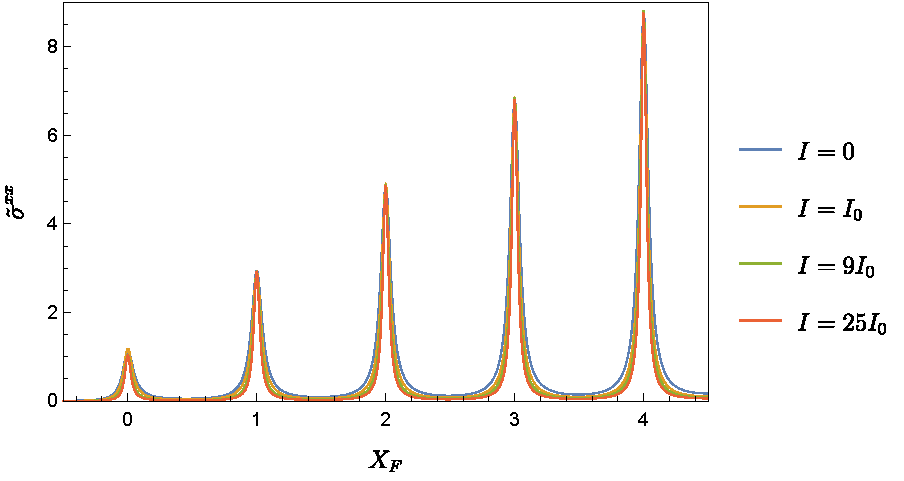
\includegraphics[scale=0.54]{figures/fig_4}
\caption{ Normalized longitudinal conductivity $\widetilde{\sigma}^{xx}$ against Fermi level $X_F$ with different intensities $I$ of the external dressing field in a GaAs-based quantum well under a nonoscillating magnetic field with $B = \SI{1.2}{\tesla}$, dressing field with a  frequency of $\omega =\SI{2e12}{\radian\per\second}$ and $I_0 =\SI{100}{\watt\per\square\centi\metre}$. In this calculation, we have assumed that the natural  broadening of $0$-th Landau level $\Gamma_0$ is $\SI{0.24}{\milli\eV}$.}
\label{fig:5}
\end{figure}

\begin{figure}[t]
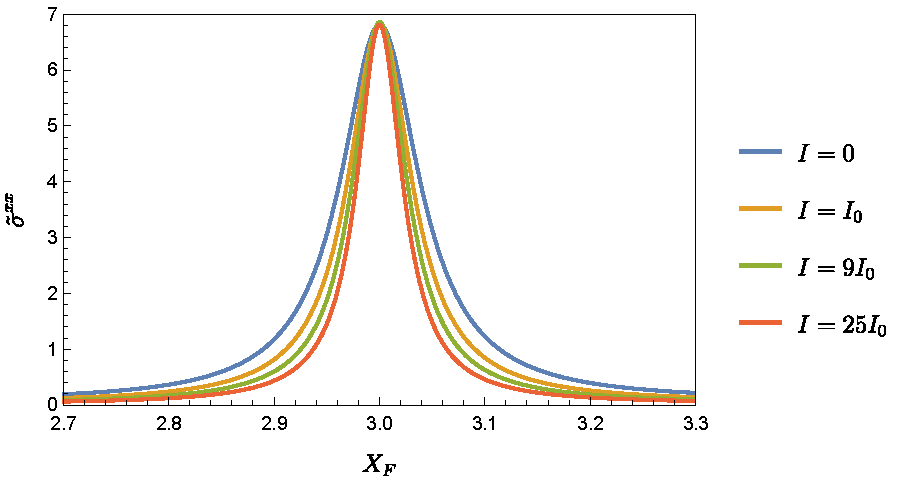
\includegraphics[scale=0.54]{figures/fig_5}
\caption{$3$rd Landau level’s normalized longitudinal conductivity $\widetilde{\sigma}^{xx}$ against Fermi level $X_F$ with different intensities $I$ of the external dressing field in a GaAs-based quantum well under a nonoscillating magnetic field with $B = \SI{1.2}{\tesla}$, dressing field with a frequency of $\omega =\SI{2e12}{\radian\per\second}$ and $I_0 =\SI{100}{\watt\per\square\centi\metre}$.
In this calculation, we have assumed that the natural  broadening of $0$-th Landau level $\Gamma_0$ is $\SI{0.24}{\milli\eV}$.}
\label{fig:6}
\end{figure}


% Section 07 :
\section{\label{sec_conclusions} Conclusions}
In this paper, we introduced a generalized mathematical model for predicting  charge transport properties in a 2DEG under a nonoscillating magnetic field and a high-intensity light. Under the uniform magnetic field, the charged particles can only settle in discrete energy values, which leads to the Landau quantization. We modeled the behavior of electrons in Landau levels under the dressing field utilizing the Floquet-Drude conductivity method. We assumed the impurities in the material as a Gaussian random scattering potential. Finally, we derived expressions for x-directional and y-directional longitudinal components of electric conductivity tensor for the considered system.

Our derived analytical expressions disclosed that the transport characteristics of the dressed quantum Hall system can be controlled by the applied dressing field’s intensity. Using detailed numerical calculations with empirical system parameters, we further analyzed the manipulation of conductivity components using the dressing field.
We found that the graphical illustrations that we obtained from these numerical calculations are capable of producing the same behavior as experiments on quantum Hall systems in the absence of a dressing field.
Furthermore, we identified that by increasing the intensity of the radiation, the conductivity regions near the Landau levels can be squeezed. Despite this behavior being identified in previous works, their results did not coincide with the more accurate description of conductivity components in undressed quantum Hall systems. However, our generalized analysis on the conductivity of dressed quantum Hall systems provide a well-suited description for these specific quantum Hall systems.

In summary, the primary purpose of this study was to broaden the modern descriptions on transport properties of dressed quantum Hall systems. Moreover, our detailed theoretical analysis showed that the recently introduced Floquet-Drude conductivity model can be adapted to extend the models that were used to describe the transport characteristics in quantum Hall systems. Owing to the ability to control the conductivity regions, high intensity external illumination may be used as a trigger for two-dimensional quantum switching devices, which are employed as the building blocks of next-generation nanoelectronic devices. As a concluding remark, we believe that our findings of this paper can be used towards understanding the 2D optoelectronic nano transistors, enhancing their performance and inventing novel appliances.


% Acknowledgments
\begin{acknowledgments}
K.H wish to acknowledge the members of A$\chi$L at Monash University for their encouragement and support and specially T.N. Perera and R.T.Wijesekara for insightful discussions. The work of K.H is supported by the Australian Government Research Training Program (RTP) Scholarship and the Monash University Institute of Graduate Research.

\end{acknowledgments}

% Add appendixes
\appendix

% Appendix A : Wave function solutions for a dressed quantum Hall system
\section{\label{appendix_a} Wave function solutions for a dressed quantum Hall system}
The derivation of the solutions for the time-dependent Schrödinger equation with our system's Hamiltonian (Eq. \ref{eq_1}) is quite similar to that followed in Refs. \cite{husimi53,dini16}. We start with expanding the Hamiltonian for two-dimensional case
\begin{equation} \label{eq_a1}
  \hat{H}_e(t) = \frac{1}{2m_e}\left[
    \left[\hat{p}_x + eBy \right]^2 +
    \left[\hat{p}_y - \frac{eE}{\omega}\cos(\omega t)\right]^2
  \right].
\end{equation}
Since $\left[\hat{H}_e(t),\hat{p}_x \right] =0$, both of these operators share same eigenfunctions
${L_x}^{-1/2}\exp(\frac{ip_x x}{\hbar})$ where $p_x = 2\pi \hbar m/L_x~$ with $ m \in \mathbb{Z}$.
Thus, we re-arrange the Hamiltonian using the definition of canonical momentum in $y$-direction and this leads to
\begin{equation} \label{eq_a2}
    \hat{H}_e(t) = \frac{1}{2m_e}\left[
      \left[{p}_x + eBy \right]^2 +
      \left[-i\hbar \pdv{y}- \frac{eE}{\omega}\cos(\omega t)\right]^2
    \right].
\end{equation}
Subsequently we define the \textit{center of the cyclotron orbit} on the $y$-axis $y_0 = {-p_x}/{eB}$ and the \textit{cyclotron frequency} $\omega_0 = {eB}/{m_e}$. This leads to a new arrangement of the Hamiltonian
\begin{equation} \label{eq_a3}
  \begin{aligned}
    \hat{H}_e(t) =
      \frac{m_e \omega_0^2}{2}\tilde{y}^2 +
      \frac{1}{2m_e}\bigg[
      -\hbar^2 \pdv[2]{\tilde{y}} & +
      \frac{2i\hbar eE}{\omega}\cos(\omega t) \pdv{\tilde{y}} \\
      & +
      \frac{e^2E^2}{\omega^2}\cos[2](\omega t)
      \bigg],
  \end{aligned}
\end{equation}
where we used a variable substitution $\tilde{y} = (y - y_0)$. Furthermore, we assume that the wave function solutions for the time-dependent Schrödinger equation of considered quantum system
\begin{equation} \label{eq_a4}
    i \hbar \dv{\psi}{t} = \hat{H}_e(t)\psi,
\end{equation}
can be presented by the following form
\begin{equation} \label{eq_a5}
    \psi_m(x,\tilde{y},t) = \frac{1}{\sqrt{L_x}} \exp\bigg(
      \frac{ip_x x}{\hbar} +
      \frac{ieE\tilde{y}}{\hbar \omega}\cos(\omega t)
    \bigg) \vartheta(\tilde{y},t),
\end{equation}
where $\vartheta(\tilde{y},t)$ is a function that satisfy the property
\begin{equation} \label{eq_a6}
    \bigg[
    \frac{m_e \omega_0^2}{2}\tilde{y}^2
    - {eE\tilde{y}}\sin(\omega t)
    -
    \frac{\hbar^2}{2m_e}
    \pdv[2]{\tilde{y}}
    - i \hbar \dv{t}
    \bigg]
    \vartheta(\tilde{y},t) = 0.
\end{equation}
If we turn off the dressing field ($E=0$), this equation leads to the Schrödinger equation with the simple harmonic oscillator Hamiltonian
\begin{equation} \label{eq_a7}
     i \hbar \dv{\vartheta(\tilde{y},t)}{t} =
    \bigg[
    \frac{\hat{p}_{\tilde{y}}^2}{2m_e} +
    \frac{1}{2}m_e \omega_0^2\tilde{y}^2
    \bigg]
    \vartheta(\tilde{y},t).
\end{equation}
Thus, we can identify $S(t) \equiv eE\sin(\omega t)$ term as an external force act on the harmonic oscillator, and we can solve this as a forced harmonic oscillator in $\tilde{y}$ axis
\begin{equation} \label{eq_a8}
  \begin{aligned}
    i \hbar \dv{\vartheta(\tilde{y},t)}{t} =
    \bigg[
    -
    \frac{\hbar^2}{2m_e}
    \pdv[2]{\tilde{y}} +
    \frac{1}{2}m_e \omega_0^2\tilde{y}^2
    - \tilde{y}S(t)]
    \bigg]
    \vartheta(\tilde{y},t).
  \end{aligned}
\end{equation}

This system is exactly solvable, and we can solve the equation using the methods explained by Husimi \cite{husimi53}. We introduce a time-dependent shifted coordinate $ y' = \tilde{y} - \zeta(t)$ and perform the following unitary transformation
\begin{equation} \label{eq_a9}
    \vartheta(y',t) = \exp(\frac{im_e\dot{\zeta}y'}{\hbar})\varphi(y',t).
\end{equation}
This leads to
\begin{equation} \label{eq_a10}
  \begin{aligned}
    i \hbar \pdv{\varphi(y',t)}{t}   &=
    \bigg[
        -  \frac{\hbar^2}{2m_e}\pdv[2]{{y'}}
        + \frac{1}{2} m_e \omega_0^2 y'^2 \\
        & +
        \Big[
            m_e\ddot{\zeta} + m_e\omega_0^2\zeta - S(t)
        \Big]y' \\
        &
        +
        \Big[
            - \frac{1}{2} m_e\dot{\zeta}^2 + \frac{1}{2}m_e\omega_0^2 \zeta^2 - \zeta S(t)
        \Big]
    \bigg]\varphi(y',t).
  \end{aligned}
\end{equation}
Subsequently, we can restrict $\zeta(t)$ function such that
\begin{equation} \label{eq_a11}
  m_e\ddot{\zeta} + m_e\omega_0^2\zeta = S(t),
\end{equation}
and that simply our previous expression as
\begin{equation} \label{eq_a12}
  \begin{aligned}
    i \hbar \pdv{\varphi(y',t)}{t}   =
    \bigg[
        -  \frac{\hbar^2}{2m_e}\pdv[2]{{y'}} &
        + \frac{1}{2} m_e \omega_0^2 {y'}^2 \\
        &
        - L(\zeta,\dot{\zeta},t)
    \bigg]\varphi(y',t).
  \end{aligned}
\end{equation}
Here
\begin{equation} \label{eq_a13}
  L(\zeta,\dot{\zeta},t) = \frac{1}{2} m_e\dot{\zeta}^2 - \frac{1}{2}m_e\omega_0^2 \zeta^2 + \zeta S(t),
\end{equation}
is the Lagrangian of a classical driven oscillator. To proceed further, another unitary transform can be introduced as follows
\begin{equation} \label{eq_a14}
    \varphi(y',t) = \exp(\frac{i}{\hbar}\int_0^{t}dt'L(\zeta,\dot{\zeta},t')) \chi(y',t),
\end{equation}
and subtitling Eq.~(\ref{eq_a14}) back in Eq.~(\ref{eq_a12}) yields
\begin{equation} \label{eq_a15}
    i \hbar \pdv{t} \chi(y',t)  =
    \bigg[
        -  \frac{\hbar^2}{2m_e}\pdv[2]{{y'}}
        + \frac{1}{2} m_e \omega_0^2 {y'}^2
    \bigg] \chi(y',t).
\end{equation}
This is the well-known Schrödinger equation of the quantum harmonic oscillator.
This allows us to identify the well known eigenfunctions \cite{griffiths18,shankar94}
\begin{equation} \label{eq_a16}
  \chi_n(y) =
   \frac{\sqrt{\kappa}}{\sqrt{2^{n}n!}}
  e^{-\kappa^2 y^2/2}
  \mathcal{H}_n \qty(\kappa y),
\end{equation}
with eigenvalues
\begin{equation} \label{eq_a17}
  \epsilon_n = \hbar \omega_0 \bigg(n + \frac{1}{2}\bigg)
  ~\text{for}~
  n \in \mathbb{Z}^{+}_0.
\end{equation}
Here, $\kappa = \sqrt{{m_e \omega_0}/{\hbar}}$, and $\mathcal{H}_n$ are the Hermite polynomials.
Thus, we can identify the solutions for Eq.~(\ref{eq_a8}) as
\begin{equation} \label{eq_a18}
  \begin{aligned}
    \vartheta_n(\tilde{y},t) = \chi_n(\tilde{y} - \zeta(t))
     \text{exp}\bigg(\frac{i}{\hbar}\bigg[&- \epsilon_nt +
    m_e\dot{\zeta(t)}\big[\tilde{y}-\zeta(t)\big] \\
     & + \int_0^{t}dt'L(\zeta,\dot{\zeta},t')\bigg]\bigg).
  \end{aligned}
\end{equation}
Since $\chi_n(x)$ functions forms a complete set, any general solution $\vartheta_(\tilde{y},t)$ can be presented with the help of the solutions derived in Eq.~(\ref{eq_a18}).

Finally, we consider our scenario where we assumed that $S(t) = eE\sin(\omega t)$, and we derive the solution for Eq.~(\ref{eq_a11}) as
\begin{equation} \label{eq_a19}
  \zeta(t) = \frac{eE}{m_e(\omega_0^2 - \omega^2)}\sin(\omega t).
\end{equation}
Subtitling solutions in Eq.~(\ref{eq_a18}) back in Eq.~(\ref{eq_a5}), we obtain a set of wave functions with two different quantum number ($n$,$m$) that satisfy the time-dependent Schrödinger equation Eq.~(\ref{eq_a4}) as follows
\begin{equation} \label{eq_a20}
  \begin{aligned}
    \psi_{n,m}&(x,y,t) \\
    &=  \frac{1}{\sqrt{L_x}}
    \chi_n\left(y - y_0 - \zeta(t)\right)\\
    &\quad\times
    \text{exp}\bigg(
    \frac{i}{\hbar}\bigg[- \epsilon_nt
    + p_x x + \frac{eE[y - y_0]}{\omega}\cos(\omega t)\\
    & \quad\quad+
    m_e\dot{\zeta}(t)\big[y - y_0 -\zeta(t)\big] +
    \int_0^{t}dt'L(\zeta,\dot{\zeta},t')\bigg]\bigg).
  \end{aligned}
\end{equation}


% Appendix B :
\section{\label{appendix_b} Floquet modes and quasienergies}
\subsection{Position space representation}

First define the time integral of Laggrangian of the classical oscillator given in Eq.~(\ref{eq_5}), over a $T=2\pi/\omega$ period as
\begin{equation} \label{eq_b1}
  \Delta_{\varepsilon} \equiv \frac{1}{T} \int_0^T dt' \; L(\zeta,\dot{\zeta},t'),
\end{equation}
and after performing the integral using Eq.~(\ref{eq_4}), we can obtain more simplified result:
\begin{equation} \label{eq_b2}
  \Delta_{\varepsilon} = \frac{(eE)^2}{4m_e(\omega_0^2 - \omega^2)}.
\end{equation}
Next define another paramter
\begin{equation} \label{eq_b3}
  \xi \equiv
  \int_0^t dt' \; L(\zeta,\dot{\zeta},t') -
  \Delta_{\varepsilon} t,
\end{equation}
and after simplying, this leads to
\begin{equation} \label{eq_b4}
  \xi =
  \frac{(eE)^2\qty(3\omega^2 - \omega_0^2)}{8m_e\omega(\omega_0^2 - \omega^2)^2} \sin(2\omega t),
\end{equation}
which is a periodic function in time with $2\omega$ frequency. Now using these  parmaters we can factorize the wavefunction Eq.~(\ref{eq_2}) as linearly time dependend part and periodic time dependend part as follows
\begin{equation} \label{eq_b5}
  \begin{aligned}
    \psi_{\alpha}(x,y,t)  = &
    \exp(\frac{i}{\hbar}\qty[-\varepsilon_nt + \Delta_{\varepsilon} t ])
    \frac{1}{\sqrt{L_x}} \chi_n\big(y - y_0 - \zeta(t)\big)
    \\
    & \times
    \text{exp}\bigg(
     \frac{i}{\hbar}\bigg[
     p_x x +
     \frac{eEy}{\omega}\cos(\omega t) \\
     & +
     m_e\dot{\zeta(t)}\big[y-\zeta(t)\big]
     + \int_0^{t}dt'L(\zeta,\dot{\zeta},t') - \Delta_{\varepsilon} t  \bigg]
     \bigg),
  \end{aligned}
\end{equation}
and this leads to seperate linear time dependent phase component as the quasienergies
\begin{equation} \label{eq_b6}
  \varepsilon_{n} =
  \hbar \omega_0\qty(n + \frac{1}{2}) - \Delta_{\varepsilon}
\end{equation}
while rest of the components as time-periodic Floquet modes
\begin{equation} \label{eq_b7}
  \begin{aligned}
    \phi_{n,m}(x,y,t) \equiv &
    \frac{1}{\sqrt{L_x}} \chi_{n}\left[y - y_0 - \zeta(t)\right]
    \text{exp}\bigg(
     \frac{i}{\hbar}\bigg[
     p_x x \\
     & +
     \frac{eE(y - y_0)}{\omega}\cos(\omega t) \\
     & +
     m_e\dot{\zeta}(t)\big[y - y_0 -\zeta(t)\big]
     + \xi \bigg]\bigg).
  \end{aligned}
\end{equation}

\subsection{Momentum space representation}

To write the Floquet modes in momentum space, we perform continuous Fourier transform over the considering confined space $A=L_xL_y$ for Eq.~(\ref{eq_7})
\begin{equation} \label{eq_b8}
  \begin{aligned}
    \phi_{n,m}(k_x,k_y,t)  &=
    \int_{-L_y/2}^{L_y/2} dy\; \exp(-i\qty[k_y - \gamma(t)]y)
    \chi_{n}\qty[y - \mu(t)] \\
     & \times
     \frac{1}{\sqrt{L_x}}
     \int_{-L_x/2}^{L_x/2} dx\;
     \exp(-ik_x x)
     \exp( \frac{i p_x }{\hbar}x ) \\
     &
     \times
     \exp(
      \frac{-i\gamma(t)}{\hbar}
      y_0)
     \exp(\frac{-i}{\hbar}
     \qty[
     m_e \dot{\zeta}(t) \zeta(t) - \xi
     ]),
  \end{aligned}
\end{equation}
where
\begin{equation} \label{eq_b9}
  \mu(t) \equiv \frac{eE\sin(\omega t)}{m_e(\omega_0^2 - \omega^2)} + y_0
  \quad,\quad
  \gamma(t) \equiv
  \frac{eE\omega_0^2\cos(\omega t)}{\hbar\omega(\omega_0^2 - \omega^2)}.
\end{equation}
Next using the identity \cite{bruus04}
\begin{equation} \label{eq_b10}
  \int_{L_x} dx\;
  \exp( -ik_x x + \frac{i p_x }{\hbar}x ) =
  L_x \delta_{k_x,\frac{p_x}{\hbar}},
\end{equation}
we can derive
\begin{equation} \label{eq_b11}
  \begin{aligned}
    \phi_{n,m}(k_x,k_y,t)  =
    \exp(
     \frac{-i\gamma(t)}{\hbar}
     y_0) &
    \exp(\frac{-i}{\hbar}
    \qty[
    m_e \dot{\zeta}(t) \zeta(t) - \xi
    ]) \\
    & \times
    \Phi_{n,m}(k_y,t)
    \delta_{k_x,\frac{p_x}{\hbar}}.
  \end{aligned}
\end{equation}
Here we defined $\Phi_{n,m}(k_y,t)$ as
\begin{equation} \label{eq_b12}
  \Phi_{n,m}(k_y,t) \equiv
  \sqrt{L_x}
  \int_{-L_y/2}^{L_y/2} dy\;
  \chi_{n}\qty[y - \mu(t)]
  \exp(
    -i\qty[k_y - \gamma(t)]
    y).
\end{equation}
Subtituting $  {k'_y} = k_y -\gamma(t)$ and $y' = y -\mu(t)$ and assuming that size of the 2DEG sample in $y$-direction is large ($L_y \rightarrow \infty$), we can obtain
\begin{equation} \label{eq_b13}
  \Phi_{n,m}({k'_y} ,t) =
  {\sqrt{L_x}} e^{-i {k'_y}\mu}
  \int_{-\infty}^{\infty} dy'\;
  \chi_{n}\qty(y')
  \exp(-i{k'_y} y').
\end{equation}
We can identify that the integral represnts the Fourier transform of $\{\chi_n\}$ functions and using the symmetric conditions \cite{celeghini21} for the Fourier transform of Gauss-Hermite functions $\theta_n(x)$:
\begin{equation} \label{eq_b14}
  \mathcal{FT}[\theta_n(\kappa x),x,k] = \frac{i^n}{|\kappa|}\theta_n(k/\kappa),
\end{equation}
Eq.~(\ref{eq_b13}) can be simplified as
\begin{equation} \label{eq_b15}
  \Phi_{n,m}({k'_y} ,t) =
    \sqrt{L_x}e^{-i {k'_y}\mu}
    \tilde{\chi}_{n}\qty({k'_y}),
\end{equation}
with
\begin{equation} \label{eq_b16}
  \tilde{\chi}_{n}\qty(k) =
  \frac{i^n}{\sqrt{2^{n} n! \sqrt{\pi}}}
  \qty(\frac{1}{\kappa})^{1/2}
  e^{-\frac{k^2}{2 \kappa^2}}
  \mathcal{H}_{\alpha} \qty(\frac{k}{\kappa}).
\end{equation}
Subtitute Eq.~(\ref{eq_b15}) back in Eq.~(\ref{eq_b11}) and this leads to
\begin{equation} \label{eq_b17}
  \begin{aligned}
    \phi_{n,m}(k_x,k_y,t)  = &
    {\sqrt{L_x}}
    \tilde{\chi}_{n}\qty(k_y - b\cos(\omega t)) \\
    & \times
    \text{exp}\left(
      i\xi
      -ik_y  \qty[d\sin(\omega t) + \frac{\hbar k_x}{eB}]
    \right),
  \end{aligned}
\end{equation}
where
\begin{equation} \label{eq_b18}
  b \equiv
  \frac{eE\omega_0^2}{\hbar\omega(\omega_0^2 - \omega^2)} \quad
  d \equiv
 \frac{eE}{m_e(\omega_0^2 - \omega^2)},
\end{equation}
and it is necessary to notice that $k_x$ is quantized with $k_x = 2\pi m/L_x ~,~ m \in \mathbb{Z}$.


% Appendix C :
\section{\label{appendix_c} Floquet-Fermi golden rule for a dressed quantum  Hall system}
The derivation of the Floquet Fermi golden rule for our quantum Hall system with the help of $t-t'$ formalism is given here in detail. The $t$-$t'$-Floquet states \cite{grifoni98,wackerl20}
\begin{equation} \label{eq_c1}
  \ket{\psi_{n,m}(t,t')} =
  \exp(-\frac{i}{\hbar}\varepsilon_{n} t)\ket{\phi_{n,m}(t')}.
\end{equation}
derived by seperating the aperiodic and periodic components of Eq.~(\ref{eq_12}), fullfill the $t$-$t'$-Schrödinger equation \cite{grifoni98,wackerl20}
\begin{equation} \label{eq_c2}
  i \hbar \pdv{t}\ket{\psi_{n,m}(t,t')} =
  H_F(t') \ket{\psi_{n,m}(t,t')},
\end{equation}
where \textit{Floquet Hamiltonian} defined as
\begin{equation} \label{eq_c3}
  H_F(t') \equiv
  H_e(t') - i\hbar \pdv{t'}.
\end{equation}
Next we can identify the the time evolution operator corresponding to the $t$-$t'$-Schrödinger equation
\begin{equation} \label{eq_c4}
  U_F(t,t_0;t') = \exp(-\frac{i}{\hbar}H_F(t')\qty[t-t_0]),
\end{equation}
and the advantage of $t$-$t'$ formalism lies on this time evolution operator which avoids any time odering operatos \cite{wackerl20}.

For our scenario, consider a time-independent total perturbation $V(\vb{r})$ which has been switched on at the reference time $t=t_0$, then the $t$-$t'$-Schrödinger equation becomes
\begin{equation} \label{eq_c5}
  i \hbar \pdv{t}\ket{\Psi_{n,m}(t,t')} =
  \qty[H_F(t') + V(\vb{r})]\ket{\Psi_{n,m}(t,t')},
\end{equation}
by introducing new wave function $\Psi_{n,m}$ for the system with the given total perturabation. If $t\leq t_0$, both solutions of the Schrödinger equations (Eq.~(\ref{eq_c2}) and Eq.~(\ref{eq_c5})) coincide
\begin{equation} \label{eq_c6}
  \ket{\psi_{n,m}(t,t')} =\ket{\Psi_{n,m}(t,t')} \quad
  \text{when} \quad
  t \leq t_0.
\end{equation}
Now move into the interaction picture representation \cite{bruus04,mahan00} of the $t$-$t'$-Floquet state
\begin{equation} \label{eq_c7}
  \ket{\Psi_{n,m}(t,t')}_I = U_0^{\dagger}(t,t_0;t')
  \ket{\Psi_{n,m}(t,t')},
\end{equation}
and due to time independency, the perturbation in the interaction picture has the same form as Schrödinger picture
\begin{equation} \label{eq_c8}
  V_I(\vb{r}) = U_0^{\dagger}(t,t_0;t')V(\vb{r})U_0(t,t_0;t') =
  V(\vb{r}).
\end{equation}
This leads to the $t$-$t'$-Schrödinger eqution in the interction picture
\begin{equation} \label{eq_c9}
  i \hbar \pdv{t}\ket{\Psi_{n,m}(t,t')}_I =
  V_I(\vb{r})\ket{\Psi_{n,m}(t,t')}_I,
\end{equation}
with the recursive solution \cite{bruus04,mahan00}
\begin{equation} \label{eq_c10}
  \begin{aligned}
  \ket{\Psi_{n,m}(t,t')}_I = &\ket{\Psi_{n,m}(t_0,t')}_I \\
  &+
  \frac{1}{i\hbar}
  \int_{t_0}^t dt_1 \;
  V_I(\vb{r}) \ket{\Psi_{n,m}(t_1,t')}_I.
  \end{aligned}
\end{equation}
Iterating the solution only upto the first order (Born approximation) we obtain
\begin{equation} \label{eq_c11}
  \begin{aligned}
    \ket{\Psi_{n,m}(t,t')}_I \approx &\ket{\psi_{n,m}(t_0,t')} \\
    &+
    \frac{1}{i\hbar}
    \int_{t_0}^t dt_1 \;
    V_I(\vb{r}) \ket{\psi_{n,m}(t_0,t')}.
  \end{aligned}
\end{equation}

In addition, since our Floquet states create a basis we can represent any solution using these Floquet states
\begin{equation} \label{eq_c12}
  \ket{\Psi_{\alpha}(t,t')} = \sum_{\beta} a_{\alpha,\beta}(t,t')
  \ket{\psi_{\beta}(t,t')}.
\end{equation}
where we used a single notation to represent two quantum numbers; $\alpha \equiv (n_{\alpha},m_{\alpha})$ and $\beta \equiv (n_{\beta},m_{\beta})$.
Then we can identify the \textit{scattering amplitude} as $a_{\alpha,\beta}(t,t') =
\braket{\psi_{\beta}(t,t')}{\Psi_{\alpha}(t,t')}$ and this can evaluate with
\begin{equation} \label{eq_c13}
  \begin{aligned}
  a_{\alpha,\beta}(t,t') = &
  \braket{\psi_{\beta}(t,t')}{\psi_{\alpha}(t,t')} \\
  &+
  \frac{1}{i\hbar}
  \int_{t_0}^t dt_1 \;
  \bra{\psi_{\beta}(t_1,t')}
  V(\vb{r}) \ket{\psi_{\alpha}(t_1,t')}.
  \end{aligned}
\end{equation}
Since the $t$-$t'$-Floquet states are orthonormal and assuming $t_0 = 0$ and $\alpha \neq \beta$ this leads to
\begin{equation} \label{eq_c14}
  a_{\alpha,\beta}(t,t') =
  -
  \frac{i}{\hbar}
  \int_{0}^t dt_1 \;
  \bra{\psi_{\beta}(t_1,t')}
  V(\vb{r}) \ket{\psi_{\alpha}(t_1,t')}.
\end{equation}

Now consider a scattering event from a $t$-$t'$-Floquet state $\ket{\psi_{\beta}(t,t')} $ into another $t$-$t'$-Floquet state $\ket{\Psi_{\alpha}(t,t')}$ with constant quansienergy $\varepsilon$:
\begin{equation} \label{eq_c15}
  \begin{aligned}
  \ket{\psi_{\beta}(t,t')} &= \exp(-\frac{i}{\hbar}\varepsilon_{\beta} t)
  \ket{\phi_{\beta}(t')} \\
  &
  \longrightarrow
  \ket{\Psi_{\alpha}(t,t')} = \exp(-\frac{i}{\hbar}\varepsilon t)
  \ket{\Phi_{\alpha}(t')}.
  \end{aligned}
\end{equation}
\begin{figure}[b]
  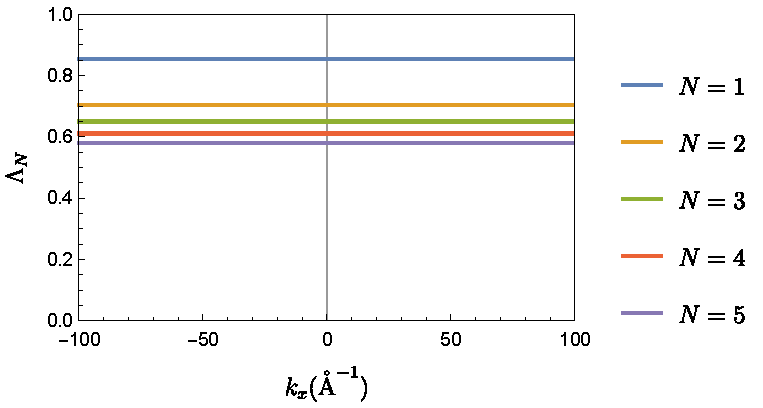
\includegraphics[scale=1.0]{figures/fig_2.pdf}
  \caption{Scattering from $\ket{\psi_{\beta}(t,t')}$ to constant energy state $\ket{\Psi_{\alpha}(t,t')}$ due to scattering potential created by impurities.}
  \label{fig_2}
\end{figure}
It is important to remember that a state of this considering system can be represented by two independent quantum numbers: $n$ represents the landau level and $m$ represents the qunatized momentum in $x$-direction. The scattering amplitutde for this scattering scenario can be calculated using the equation derived in Eq.~(\ref{eq_c14})
\begin{equation} \label{eq_c16}
  \begin{aligned}
    a_{\alpha\beta}(t,t') =
    -\frac{i}{\hbar}
    \int_{0}^t dt_1 \;
    e^{\frac{i}{\hbar}\qty(\varepsilon_{\beta} - \varepsilon)t_1}
    \bra{\phi_{\beta}(t')}
    V(\vb{r}) \ket{\phi_{\alpha}(t')},
  \end{aligned}
\end{equation}
and assuiming for a long time $t \rightarrow \infty$, we can turn this integral into a delta distrubution
\begin{equation} \label{eq_c17}
  \begin{aligned}
    a_{\alpha\beta}(t') =
    -2\pi i \delta(\varepsilon_{\beta} - \varepsilon)Q,
  \end{aligned}
\end{equation}
where $Q \equiv \bra{\phi_{\beta}(t')}
V(\vb{r}) \ket{\phi_{\alpha}(t')}$ and using completeness properties we can re-write this as
\begin{equation} \label{eq_c18}
    Q =
    \sum_{\vb{k}}\sum_{\vb{k'}}
    \braket{\phi_{\beta}(t')}{\vb{k'}}
    \mel{\vb{k'}}{V(\vb{r})}{\vb{k}}
    \braket{\vb{k}}{\phi_{\alpha}(t')},
\end{equation}
and seperating $x$ and $y$ directional momentums we can derive (we already assumed that $L_y \rightarrow \infty$)
\begin{equation} \label{eq_c19}
    Q =
    \sum_{k_x}\sum_{{k'}_x}
    \int_{-\infty}^{\infty} \int_{-\infty}^{\infty} dk_y d{k'}_y \;
    V_{\vb{k'},\vb{k}}
    \phi_{\beta}^{\dagger}(\vb{k'},t')
    \phi_{\alpha}(\vb{k},t').
\end{equation}
with $V_{\vb{k'},\vb{k}} \equiv \mel{\vb{k'}}{V(\vb{r})}{\vb{k}}$.

Since the perturbation potential $V(\vb{r})$ is assumed to be formed by an ensemble of randomly distributed impurities, consider $N_{imp}$ identical impurities positioned at randomly distributed but fixed positions $\vb{r}_i$. Then scattering potential $V(\vb{r})$ is given by the sum over uncorrelated single impurity potentials $\upsilon(\vb{r})$
\begin{equation} \label{eq_c20}
  V(\vb{r}) \equiv
  \sum_{i=1}^{N_{imp}}
  \upsilon (\vb{r}-\vb{r}_i).
\end{equation}
Next we model the perturbation $V(\vb{r})$ as a Gaussian random potential where one can choose the zero of enerrgy such that the potential is zero on average. This model is characterized by \cite{akkermans10}
\begin{subequations}
\begin{equation} \label{eq_c21a}
  \expval{\upsilon(\vb{r})}_{imp} =0,
\end{equation}
\begin{equation} \label{eq_c21b}
  \expval{\upsilon(\vb{r})\upsilon(\vb{r'})}_{imp} = \Upsilon(\vb{r}-\vb{r'}),
\end{equation}
\end{subequations}
where $\expval{\cdot}_{imp}$ denoted the average over realizations of the impurity disorder and $\Upsilon(\vb{r}-\vb{r'})$ is any decaying function depends only on $\vb{r}-\vb{r'}$. In addition, this model assume that $\upsilon (\vb{r}-\vb{r'})$ only dependes on the position difference $|\vb{r}-\vb{r'}|$ and it decays with a characteristic leangth $r_c$. Since this study considers the case where the waveleagth of radiation or scattering electrons is much faster than $r_c$, it is a good approximation to make two-point correlation function to be
\begin{equation} \label{eq_c22}
  \expval{\upsilon(\vb{r})\upsilon(\vb{r'})}_{imp} = \Upsilon_{imp}^2\delta(\vb{r}-\vb{r'}),
\end{equation}
where $\Upsilon_{imp}$ is stregth of the delta potential and a random potential $V(\vb{r})$ with this property is called white noise \cite{akkermans10}. Then we can model approximately the total scattering potential as
\begin{equation} \label{eq_c23}
  V(\vb{r}) =
  \sum_{i=1}^{N_{imp}}
  \Upsilon_{imp} \delta(\vb{r}-\vb{r}_i).
\end{equation}
Then we can calculate $V_{\vb{k'},\vb{k}}$ using this assumption as follows
\begin{subequations} \label{eq_c24}
\begin{align}
 V_{\vb{k'},\vb{k}} & =
 \mel**{\vb{k'}}{\sum_{i=1}^{N_{imp}}
 \Upsilon_{imp} \delta(\vb{r}-\vb{r}_i)}{\vb{k}} \label{eq_c24a} \\
 & =
 \sum_{i=1}^{N_{imp}}
 \int_{-\infty}^{\infty} dy\; \bigg[
 \frac{1}{\sqrt{L_xL_y}} e^{ik'_y y} \delta(y-y_i) \nonumber \\
 & \times \frac{1}{\sqrt{L_xL_y}} e^{-i{k}_y y}
 \mel**{k'_x}{\Upsilon_{imp} \delta(x-x_i)}{k_x} \bigg] \label{eq_c24b} \\
  & =
 \sum_{i=1}^{N_{imp}} \frac{1}{{L_xL_y}}
 e^{i(k'_y - k_y )y}
 \mel**{k'_x}{\Upsilon_{imp} \delta(x-x_i)}{k_x} \label{eq_c24c}.
\end{align}
\end{subequations}
Since $\upsilon (\vb{r})$ in momentum space is a constant value, each impurity  produce same impurity potential for every $x$-directional momentum pairs and assuming the total ncumber of scatterers $N_{imp}$ is macroscopically large, we can derive
\begin{subequations} \label{eq_c25}
  \begin{align}
    V_{\vb{k'},\vb{k}}
    & =
    V_{k'_x,k_x}
    \frac{N_{imp}}{L_y L_x} \int_{-\infty}^{\infty} dy_i\;
    e^{i\qty({k'}_y - k_y)y_i} \label{eq_c25a} \\
    & =
    \eta_{imp} V_{k'_x,k_x} \delta(k'_y - k_y), \label{eq_c25b}
  \end{align}
\end{subequations}
where
\begin{equation} \label{eq_c26}
  V_{{k'}_x,k_x} \equiv
  \mel**{k'_x}{\Upsilon_{imp} \delta(x-x_i)}{k_x}.
\end{equation}
is a constant value for every $i$ impurity and $\eta_{imp}$ is number of impurities in a unit area. It is important to notice that $\ket{k_x} = e^{-ik_xx}$.

Now using Eq.~(\ref{eq_9}) and Eq.~(\ref{eq_c25}) on Eq.~(\ref{eq_c19}), we obtain (with changing varable $t' \rightarrow t'$)
\begin{equation} \label{eq_c27}
  \begin{aligned}
    Q & =
    \sum_{k_x}\sum_{{k'}_x}
    {\eta_{imp} V_{{k'}_x,k_x}}
    \int_{-\infty}^{\infty} \int_{-\infty}^{\infty} dk_y d{k'}_y \;
    \delta({k'}_y - k_y)
    \\
    & \times
    \sqrt{L_x}
    \exp(
      i{k'}_y  \qty[d\sin(\omega t) + {y'}_0]
    )
    \tilde{\chi}_{n_{\beta}}\qty({k'}_y -b\cos(\omega t))
    \\
    & \times
    \sqrt{L_x}
    \exp(
      -ik_y  \qty[d\sin(\omega t) + y_0]
    )
    \tilde{\chi}_{n_{\alpha}}\qty(k_y -b\cos(\omega t)),
  \end{aligned}
\end{equation}
and this can simplify as
\begin{equation} \label{eq_c28}
  \begin{aligned}
    Q =
    \sum_{k_x}\sum_{{k'}_x}
    {\eta_{imp} L_x V_{{k'}_x,k_x}} I,
  \end{aligned}
\end{equation}
with
\begin{equation} \label{eq_c29}
  \begin{aligned}
    I \equiv
    \int_{-\infty}^{\infty} dk_y \;
    \tilde{\chi}_{n_{\beta}}\qty(k_y -b\cos(\omega t)) &
    \tilde{\chi}_{n_{\alpha}}\qty(k_y -b\cos(\omega t)) \\
    & \times
    \exp(
      -ik_y  \qty[y_0 - {y'}_0  ]
    ).
  \end{aligned}
\end{equation}
To avoid the energy exchange from external strong field and electrons, the applied radiation should be a purely dressing field. Therefore, the only effect of the dressing field on 2DEG is the renormalization of the probability of elastic electron scattering within the same Landau level $(n_{\alpha} = n_{\beta} =N)$. This transform the Eq.~(\ref{eq_c29}) to
\begin{equation} \label{eq_c30}
    I =
    \int_{-\infty}^{\infty} dk_y \;
    \tilde{\chi}_{N}^2 \qty(k_y -b\cos(\omega t))
    \exp(
      -ik_y  \qty[y_0 - {y'}_0  ]
    ).
\end{equation}
Using Fourier transform of Gauss-Hermite functions \cite{celeghini21} and convolution theorem \cite{arfken85,bracewell78} we can derive
\begin{equation} \label{eq_c31}
  \begin{aligned}
    I =
    {2\pi} &
    \exp(b[{y'}_0 - y_0]\cos(\omega t)) \\
    & \times
    \int_{-\infty}^{\infty} dy \;
    {\chi}_{N}\qty(y)
    {\chi}_{N}\qty(y_0 - {y'}_0 - y).
  \end{aligned}
\end{equation}
Therefore finally the scattering amplitude derived in Eq.~(\ref{eq_c17}) can be evaluated for given $k_x = 2\pi m_{\alpha}/L_x$ and $k'_x =  2\pi m_{\beta}/L_x$ as
\begin{equation} \label{eq_c32}
  \begin{aligned}
    a_{\alpha\beta}(k_x,k'_x,t)  =&
    -2\pi i
    \eta_{imp} L_x V_{{k'}_x,k_x}
    \delta(\varepsilon_{N} - \varepsilon)\\
    & \times
    \exp(b[{y'}_0 - y_0]\cos(\omega t))\\
    & \times
    \int_{-\infty}^{\infty} dy \;
    {\chi}_{N}\qty(y)
    {\chi}_{N}\qty(y_0 - {y'}_0 - y),
  \end{aligned}
\end{equation}
Since this scattering amplitude is time-periodic we can write this as a Fourier series expansion
\begin{equation} \label{eq_c33}
    a_{\alpha\beta}(k_x,k'_x,t) =
    \sum_{l=-\infty}^{\infty} a^l_{\alpha\beta}(k_x,k'_x) e^{-il\omega t}.
\end{equation}
In addition, using Jacobi-Anger expansion \cite{cuyt08,abramowitz64}
\begin{equation} \label{eq_c34}
    e^{iz\cos(\theta)} = \sum_{l=-\infty}^{\infty} i^l J_l\qty(z) e^{-il\theta},
\end{equation}
where $J_l(z)$ are Bessel functions of the first kind with $l$-th integer order and we can re-write the Eq.~(\ref{eq_c32}) as folllows
\begin{equation} \label{eq_c35}
  \begin{aligned}
    a_{\alpha\beta}(k_x,k'_x,t)  = &
    \sum_{l=-\infty}^{\infty}
    -2\pi i^{l+1}
    \eta_{imp} L_x V_{{k'}_x,k_x}
    \delta(\varepsilon_{N} - \varepsilon)\\
    & \times
    J_l\qty(b[{y'}_0 - y_0]) \\
    & \times
    \int_{-\infty}^{\infty} dy \;
    {\chi}_{N}\qty(y)
    {\chi}_{N}\qty(y_0 - {y'}_0 - y) e^{-il\omega t},
  \end{aligned}
\end{equation}
and then the Fourier series component can be identified as
\begin{equation} \label{eq_c36}
  \begin{aligned}
    a^l_{\alpha\beta}(k_x,k'_x) = &
    -2\pi i^{l+1}
    \eta_{imp} L_x V_{{k'}_x,k_x}\\
    & \times
    \delta(\varepsilon_{N} - \varepsilon)
    J_l\qty(b[{y'}_0 - y_0])\\
    & \times
    \int_{-\infty}^{\infty} dy \;
    {\chi}_{n_{\beta}}\qty(y)
    {\chi}_{n_{\beta}}\qty(y_0 - {y'}_0 - y).
  \end{aligned}
\end{equation}
Now define \textit{transition probability matrix}
\begin{equation} \label{eq_c37}
    \qty(A_{\alpha\beta})_{l,l'} \equiv
    a^l_{\alpha\beta}\qty[a^{l'}_{\alpha\beta}]^{*},
\end{equation}
and this becomes
\begin{equation} \label{eq_c38}
  \begin{aligned}
      \qty(A_{\alpha\beta})_{l,l'}(k_x,k'_x) = &
      \qty[{ 2 \pi \eta_{imp} L_x |V_{{k'}_x,k_x}|}]^2
      \delta^2(\varepsilon_{N} - \varepsilon) \\
      & \times
      J_l\qty(b[{y'}_0 - y_0]) J_{l'}\qty(g[{y'}_0 - y_0])\\
      & \times
      \qty|
      \int_{-\infty}^{\infty} dy \;
      {\chi}_{n_{\beta}}\qty(y)
      {\chi}_{n_{\beta}}\qty(y_0 - {y'}_0 - y)|^2.
  \end{aligned}
\end{equation}
Then desribing the square of the delta distribution using following procedure \cite{dini16,kibis14}
\begin{equation} \label{eq_c39}
    \delta^2(\varepsilon) =
    \delta(\varepsilon)\delta(0) =
    \frac{\delta(\varepsilon)}{2\pi \hbar}
    \int_{-t/2}^{t/2} e^{i0\times t'/\hbar} dt'\; =
    \frac{\delta(\varepsilon)t}{2\pi \hbar},
\end{equation}
and performing the time derivation of each matrix element yeild the \textit{transition amplitude matrix}:
\begin{equation} \label{eq_40}
  \begin{aligned}
    \Gamma_{\alpha\beta}^{ll'}(k_x,k'_x) = &
    \frac { 2\pi \eta_{imp}^2 L_x^2}{ \hbar} |V_{{k'}_x,k_x}|^2
    \delta(\varepsilon_{\beta} - \varepsilon)\\
    & \times
    J_l\qty(b[{y'}_0 - y_0]) J_{l'}\qty(g[{y'}_0 - y_0]) \\
    & \times
    \qty|
    \int_{-\infty}^{\infty} dy \;
    {\chi}_{N}\qty(y)
    {\chi}_{N}\qty(y_0 - {y'}_0 - y)|^2.
  \end{aligned}
\end{equation}

An impurity average of white noise potential allows to identify $\expval{|V_{{k'}_x,k_x}|^2} = V_{imp}$ and the inverse scattering time matrix is the sum over all momentum over the transition probability matrix
\begin{equation} \label{eq_41}
    \qty(\frac{1}{\tau(\varepsilon,k_x)})^{ll'}_{\alpha\beta} \equiv
    \frac{1}{L_x} \sum_{{k'}_x}
    \expval**{\Gamma_{\alpha\beta}^{ll'}({k'}_x,k_x)}_{imp},
\end{equation}
and applying the 1-dimentional momentum continuum limit $\sum_{{k'}_x} \longrightarrow {L_x}/{2\pi}\int d {k'}_x$ and this leads to
\begin{equation} \label{eq_42}
  \begin{aligned}
    \bigg(&\frac{1}{\tau(\varepsilon,k_x)}\bigg)^{ll'}_{\alpha\beta} \\
    & =
    \frac { 2\pi \eta_{imp}^2 L_x^2}{ \hbar}
    \frac{V_{imp}}{2\pi}
    \delta(\varepsilon_{\beta} - \varepsilon)\\
    & =
    \int_{-\infty}^{\infty} d {k'}_x
    J_l\qty(\frac{b\hbar}{eB}[{k}_x - {k'}_x])
    J_{l'}\qty(\frac{b\hbar}{eB}[{k}_x - {k'}_x]) \\
    & \times
    \qty|
    \int_{-\infty}^{\infty} dy \;
    {\chi}_{n_{\beta}}\qty(y)
    {\chi}_{n_{\beta}}\qty(\frac{\hbar}{eB} \qty[{k'}_x - {k}_x] - y)|^2.
  \end{aligned}
\end{equation}
Using subtitution $k'_x = k_1$ and $y = {\hbar{k_2}}/{eB}$ finally we can derive our expression for the inverse scattering time matrix for $N$-th Landau
level
\begin{equation} \label{eq_43}
  \begin{aligned}
    \bigg(&\frac{1}{\tau(\varepsilon,k_x)}\bigg)^{ll'}_{N} \\
    & =
    \frac { \eta_{imp}^2 L_x^2 \hbar V_{imp}}{\qty(eB)^2}
    \delta(\varepsilon - \varepsilon_{N})\\
    & \times
    \int_{-\infty}^{\infty} d k_1
    J_l\qty(\frac{b\hbar}{eB}[{k}_x - k_1])
    J_{l'}\qty(\frac{b\hbar}{eB}[{k}_x - k_1]) \\
    & \times
    \qty|
    \int_{-\infty}^{\infty} dk_2 \;
    {\chi}_{N}\qty(\frac{\hbar}{eB}k_2)
    {\chi}_{N}\qty(\frac{\hbar}{eB} \qty[k_1 - {k}_x - k_2])|^2.
  \end{aligned}
\end{equation}


% Appendix D :
\section{\label{appendix_d} Current operators for a dressed quantum Hall system}
In this section we are hoping to derive the current density operator for $N$-th Landau level. We already found the extact solution for our time depenedent Hamiltonian Eq.~(\ref{eq_1}) and we identified them as Floquet states with quesienergies Eq.~(\ref{eq_12}). The Floquet modes derived in Eq. Eq.~(\ref{eq_9}) can be represented as states using quantum number for the simplicity of notation as follows
\begin{equation} \label{eq_d1}
  \ket{\phi_{n,m}} \equiv \ket{n,k_x}
\end{equation}
Using above complete set of eigenstates of Floquet Hamiltonian Eq.~(\ref{eq_c3}) \cite{wackerl20,holthaus15,grifoni98} we can represent the single particle current operator's matrix element as
\begin{equation} \label{eq_d2}
  \qty(\vb{j})_{nm,n'm'} \equiv \mel{n,k_x}{\;\hat{\vb{j}}\;}{n',k'_x},
\end{equation}
and particle current operator for our system \cite{mahan00,bruus04} by
\begin{equation} \label{eq_d3}
  \hat{\vb{j}} = \frac{1}{m} \qty(\hat{\vb{p}} - e\qty[\vb{A}_s + \vb{A}_d(t)]).
\end{equation}
where $m$ is mass of the considering particle.

First consider the transverse conductivity in $x$-direction and we can identify that $x$-directional current operator as
\begin{equation} \label{eq_d4}
  \hat{j}_x = \frac{1}{m} \qty(-i\hbar\pdv{x} + eBy).
\end{equation}
Now calculate the matrix elements of $x$-directional current operator in Floquet mode basis
\begin{equation} \label{eq_d5}
  \qty({j}_x)_{nm,n'm'} =
  \mel{n,k_x}{\;\frac{1}{m} \qty(-i\hbar\pdv{x} + eBy)\;}{n',k'_x}.
\end{equation}
Then evaluate these using Floquet modes derived in Eq.~(\ref{eq_7}) and obtain
\begin{equation} \label{eq_d6}
  \begin{aligned}
    \qty({j}_x)_{nm,n'm'} = &
    \frac{1}{{m}}
    \delta_{k_x,k'_x}
    \int dy \;
    \Big[
    \qty(\hbar k'_x + eBy) \\
    & \times
     \chi_{n}\big(y - y_0 - \zeta(t)\big)
    \chi_{n'}\big(y - y_0 - \zeta(t)\big)
    \Big].
  \end{aligned}
\end{equation}
Then let $y - y_0 - \zeta(t) = \bar{y}$ and we can derive
\begin{equation} \label{eq_d7}
  \begin{aligned}
    \qty({j}_x)_{nm,n'm'} =
    \frac{1}{{m}}
    \delta_{k_x,k'_x}
    \int d\bar{y} \;
    \Big[ &
    \qty(\hbar k'_x + eB\bar{y} -\hbar k'_x + eB\zeta(t)) \\
    & \times
    \chi_{n}(\bar{y})
    \chi_{n'}(\bar{y})
    \Big].
  \end{aligned}
\end{equation}
Using following integral identities of Floquet modes which are made up with  Gauss-Hermite functions \cite{vedenyapin11,szego59}
\begin{subequations} \label{eq_d8}
  \begin{align}
    \int d{y} \;
    \chi_{n}({y})
    \chi_{n'}({y}) &=
    \delta_{n',n} \\
    \int dy \;
    y
    \chi_{n}({y})
    \chi_{n'}({y}) &=
    \qty(\sqrt{\frac{n+1}{2}} \delta_{n',n+1} + \sqrt{\frac{n}{2}}
    \delta_{n',n-1}),
  \end{align}
\end{subequations}
we simplfy the matrix elements of $x$-directional current operator to
\begin{equation} \label{eq_d9}
  \begin{aligned}
    \qty({j}_x)_{nm,n'm'} =
    \frac{1}{{m}}
    \delta_{k_x,k'_x}
    eB
    \bigg[
    \bigg(\sqrt{\frac{n+1}{2}} \delta_{n',n+1} & + \sqrt{\frac{n}{2}}
    \delta_{n',n-1}\bigg) \\
    &
    + \zeta(t) \delta_{n',n}
    \bigg]
  \end{aligned}
\end{equation}

Due to high complexity of extract solution, in this study we only consider the constant contribution. Therefore we evaluate the $s=0$ component of the Fourier series with
\begin{equation} \label{eq_d10}
    \qty({j}^x_{s=0})_{nm,n'm'} =
    \frac{eB}{{m}}
    \delta_{k_x,k'_x}
    \qty(\sqrt{\frac{n+1}{2}} \delta_{n',n+1} + \sqrt{\frac{n}{2}}
    \delta_{n',n-1}).
\end{equation}
For electric current operator we can apply the electron's charge and effective mass and this leads to
\begin{equation} \label{eq_d11}
    \Big({j}^x_{s=0}\Big)_{nm,n'm'}^{elctron} =
    \frac{e^2B}{{m_e}}
    \delta_{k_x,k'_x}
    \qty(\sqrt{\frac{n+1}{2}} \delta_{n',n+1} + \sqrt{\frac{n}{2}}
    \delta_{n',n-1}).
\end{equation}

Next we consider the transverse conductivity in $y$-direction and we can identify that $y$-directional current operator as
\begin{equation} \label{eq_d12}
  \hat{j}_y = \frac{1}{m} \qty(-i\hbar\pdv{y} - \frac{eE}{\omega}\cos(\omega t)).
\end{equation}
Then the matrix elements of $y$-directional current operator in Floquet mode basis are derived as
\begin{equation} \label{eq_d13}
  \qty({j}_y)_{nm,n'm'} =
  \mel{n,k_x}{\;\frac{-1}{m} \qty(i\hbar\pdv{y} + \frac{eE}{\omega}\cos(\omega t))\;}{n',k'_x}.
\end{equation}
After following the same steps done for $x$-directional current operator, we can derive the $s=0$ component of matrix elements for $y$-directional electric current operator
\begin{equation} \label{eq_d14}
    \Big({j}^y_{s=0}\Big)_{nm,n'm'}^{elctron} =
    \frac{ie\hbar}{{m_e}}
    \delta_{k_x,k'_x}
    \qty[
    \sqrt{\frac{n}{2}} \delta_{n',n-1}
    - \sqrt{\frac{n+1}{2}} \delta_{n',n+1}
    ].
\end{equation}









x


% Bibliography
\bibliography{aps_article}

\end{document}

% ****** End of file dressed_quantum_hall.tex ****** %
